
In the following section, the values for relative GIA produced by this paper are
contrasted with those previously obtained by Mainville \& Craymer by plotting the
difference between each site as a line between sites with the corresponding value
next to it on a map.

\begin{figure}[h]
	\makebox[\textwidth]{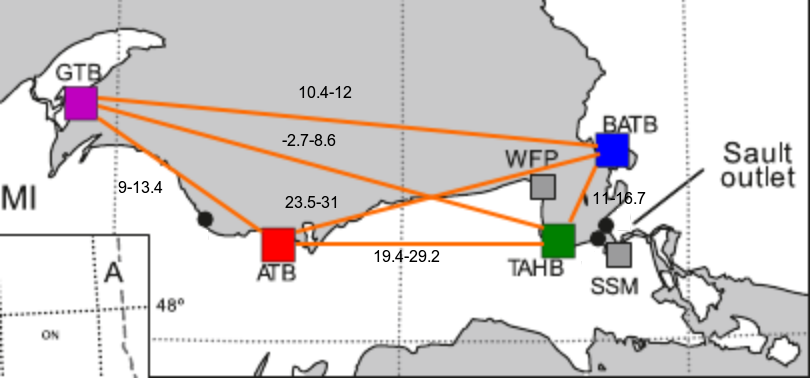
\includegraphics[width=0.72\paperwidth]{johnstonLaurentianMapWithMyGIARates.png}}
	\caption{Relative GIA Rates produced by this papers method, all values reported in cm/century}
	\label{fig:myGIARates}
\end{figure}
\newpage
\begin{figure}[h]
	\makebox[\textwidth]{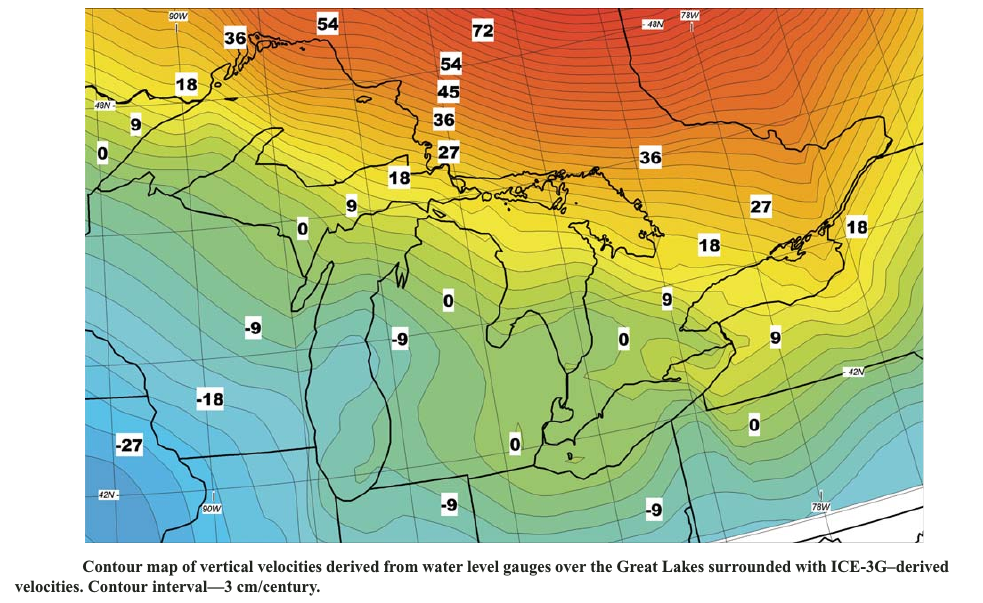
\includegraphics[width=0.72\paperwidth]{mainvilleGias.png}}
	\caption{Relative GIA Rates produced by Mainville \& Craymer, all values reported in cm/century (reproduced from Mainville \& Craymer, 2005)}
	\label{fig:craymerGIARatesBigPlot}
\end{figure}

The equivalent values for rates between sites as produced by Mainville \& Craymer
are inferred from subtracting the difference in contour between sites as shown in
Figure \ref{fig:craymerGIARatesBigPlot}, and are presented in Figure \ref{fig:craymerGIARates}.

\begin{figure}[h]
	\makebox[\textwidth]{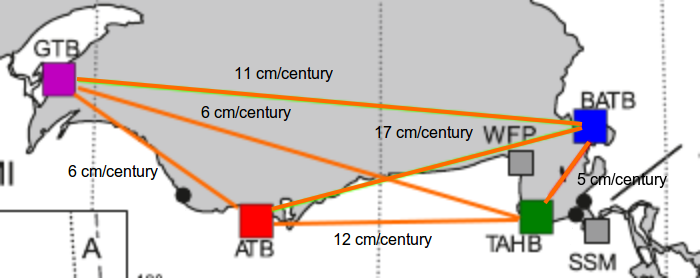
\includegraphics[width=0.72\paperwidth]{johnstonLaurentianMapWithCraymerGIARates.png}}
	\caption{Relative GIA Rates produced by Mainville \& Craymer}
	\label{fig:craymerGIARates}
\end{figure}
\newpage

While most of the site comparisons agree reasonably well between the method
employed by Mainville \& Craymer and this paper, one area where significant
disagreement is seen is between sites ATB, BATB, and TAHB, especially in the much
larger values produced by this paper between ATB-BATB and ATB-TAHB. Given that both
of these site combinations are separated by an East-West line, this could imply
that the location of the center of the Laurentide Ice Sheet during the last glaciation being to the
north and west of Lake Superior had a stronger effect on the overall process of
rebound than the simple fact that areas to the north were more likely to be
depressed by the weight of ice sheets than areas further south.
